%%%%%%%%%%%%%%%%%%%%%%%%%%%%%%%%%%%%%%%%%
% Short Sectioned Assignment LaTeX Template Version 1.0 (5/5/12)
% This template has been downloaded from: http://www.LaTeXTemplates.com
% Original author:  Frits Wenneker (http://www.howtotex.com)
% License: CC BY-NC-SA 3.0 (http://creativecommons.org/licenses/by-nc-sa/3.0/)
%%%%%%%%%%%%%%%%%%%%%%%%%%%%%%%%%%%%%%%%%

%----------------------------------------------------------------------------------------
%	PACKAGES AND OTHER DOCUMENT CONFIGURATIONS
%----------------------------------------------------------------------------------------

\documentclass[paper=a4, fontsize=11pt]{scrartcl} % A4 paper and 11pt font size

% ---- Entrada y salida de texto -----

\usepackage[T1]{fontenc} % Use 8-bit encoding that has 256 glyphs
\usepackage[utf8]{inputenc}
%\usepackage{fourier} % Use the Adobe Utopia font for the document - comment this line to return to the LaTeX default

% ---- Idioma --------

\usepackage[spanish, es-tabla]{babel} % Selecciona el español para palabras introducidas automáticamente, p.ej. "septiembre" en la fecha y especifica que se use la palabra Tabla en vez de Cuadro

% ---- Otros paquetes ----

\usepackage{url} % ,href} %para incluir URLs e hipervínculos dentro del texto (aunque hay que instalar href)
\usepackage{amsmath,amsfonts,amsthm} % Math packages
%\usepackage{graphics,graphicx, floatrow} %para incluir imágenes y notas en las imágenes
\usepackage{graphics,graphicx, float} %para incluir imágenes y colocarlas

\usepackage{enumitem}

% Para hacer tablas comlejas
%\usepackage{multirow}
%\usepackage{threeparttable}

% Para utilizar pseudocódigo
\usepackage{algorithm}
\usepackage{algorithmic}
\usepackage{algorithmicx}
\usepackage{listings}

%\usepackage{sectsty} % Allows customizing section commands
%\allsectionsfont{\centering \normalfont\scshape} % Make all sections centered, the default font and small caps

\usepackage{fancyhdr} % Custom headers and footers
\pagestyle{fancyplain} % Makes all pages in the document conform to the custom headers and footers
\fancyhead{} % No page header - if you want one, create it in the same way as the footers below
\fancyfoot[L]{} % Empty left footer
\fancyfoot[C]{} % Empty center footer
\fancyfoot[R]{\thepage} % Page numbering for right footer
\renewcommand{\headrulewidth}{0pt} % Remove header underlines
\renewcommand{\footrulewidth}{0pt} % Remove footer underlines
\setlength{\headheight}{13.6pt} % Customize the height of the header

\numberwithin{equation}{section} % Number equations within sections (i.e. 1.1, 1.2, 2.1, 2.2 instead of 1, 2, 3, 4)
\numberwithin{figure}{section} % Number figures within sections (i.e. 1.1, 1.2, 2.1, 2.2 instead of 1, 2, 3, 4)
\numberwithin{table}{section} % Number tables within sections (i.e. 1.1, 1.2, 2.1, 2.2 instead of 1, 2, 3, 4)

\setlength\parindent{0pt} % Removes all indentation from paragraphs - comment this line for an assignment with lots of text

\newcommand{\horrule}[1]{\rule{\linewidth}{#1}} % Create horizontal rule command with 1 argument of height


%----------------------------------------------------------------------------------------
%	TÍTULO Y DATOS DEL ALUMNO
%----------------------------------------------------------------------------------------

\title{	
\normalfont \normalsize 
\textsc{\textbf{Metaheurística} \\ Doble Grado en Ingeniería Informática y Matemáticas \\ Universidad de Granada} \\ [25pt] % Your university, school and/or department name(s)
\horrule{0.5pt} \\[0.4cm] % Thin top horizontal rule
\Huge Práctica 1\\
\LARGE Metaheurísticas novedosas: Brain Storm Optimization
 \\ % The assignment title
\horrule{2pt} \\[0.5cm] % Thick bottom horizontal rule
}

\author{ Iván Sevillano García \\\\
	DNI: 77187364-P\\ \\
	E-mail: ivansevillanogarcia@correo.ugr.es\\\\
	} % Nombre y apellidos

\date{\normalsize\today} % Incluye la fecha actual

%----------------------------------------------------------------------------------------
% DOCUMENTO
%----------------------------------------------------------------------------------------

\begin{document}

\maketitle % Muestra el Título

\newpage

\tableofcontents
\newpage

\section{Presentación de la metaheurística. Problema que soluciona.}

Esta metaheurística la comenzó a desarrollar Yuhui Shi en la universidad de Liverpool\cite{BSO}. Está basada en la idea de que el desarrollo de soluciones para problemas de distinta índole se basa en el desarrollo de una lluvia de ideas, las cuales se pueden ir mejorando con distintos mecanismo. \\

Esta idea surgió porque las metaheurísticas bio-inspiradas han dado buenos resultados en distintos campos. Las que se basan en poblaciones, por ejemplo, se basan en paralelismos con peces, hormigas, pájaros, peces... Y siendo el ser humano un ser vivo más (y, según el paper, el más inteligente), ¿Por qué no utilizar su forma de llegar a soluciones óptimas a problemas para resolver problemas de optimización?\\

\subsection{Proceso humano de la lluvia de ideas. Modelo abstracto.}

El mecanismo de lluvia de ideas para generar ideas para un proyecto es muy conocido. En él se genera entre todos los individuos tantas ideas como se pueda para luego trabajar sobre ellas e intentar encaminar la búsqueda de la mejor solución. El algoritmo que describen en el paper sería el siguiente:\\

\begin{enumerate}
	\item Generamos ideas de distinta índole sin importar lo buenas o malas que sean a priori.
	\item Sobre estas ideas, seleccionamos unas pocas ideas buenas que sean representativas del resto de ideas. Estas ideas tendrán más probabilidad de ser seleccionadas para ser mejoradas.
	\item Se intenta potenciar las ideas seleccionadas con más probabilidad tanto mezclando con otras como profundizando en la misma.
	\item Con suerte, se habrá generado una idea lo suficientemente buena. Se puede repetir el proceso de optimización de ideas tantas veces se quiera o se pueda.
\end{enumerate}

Cuando utilizamos la idea de idea representante y le damos más prioridad la utilizamos para que se utilice esta idea como un punto atractor del resto. Puesto que tiene mejor puntuación, debe de ser una idea entorno a la cuál profundizar la búsqueda de soluciones óptimas. También, como diferenciamos entre distintos representantes, actúan como distintos puntos atractores, manteniendo la búsqueda diversificada.


La creación de ideas sigue unas reglas descritas en el paper referidas a las regalse descritas en \cite{smith}, las cuales se detallan a continuación: 

\begin{itemize}
	\item Ninguna idea, a priori, es mala
	\item Todo lo que se ocurra será productivo para la generación de la idea optimizada.
	\item La generación de nuevas ideas deben generarse en base a ideas previas generadas.
	\item Prioriza la cantidad, la calidad vendrá a sola.
\end{itemize}

Estas reglas se crean para generar tantas ideas como podamos y para que estas tengan mucha diversidad. Cuantas más ideas tengamos, más posibilidad tendremos de encontrar mejores soluciones.\\

\newpage

\section{Breve descripción de los algorítmos utilizados.}

Tras la introducción abstracta de la lluvia de ideas, veamos cómo formalizar este procedimiento para la optimización de parámetros. Para empezar, desarrollaremos los paralelismos:\\

\begin{itemize}
	\item \textbf{Idea}. El concepto de idea lo transportamos al de solución, que para la optimización de parámetros será un vector de tantos elementos reales como dimensión del problema.
	
	\item \textbf{Generación de ideas aleatorias.} Generaremos ideas generando vectores aleatorios dentro del conjunto donde buscamos.
	
	\item \textbf{Ideas semejantes.} Para separar ideas por "semejanza", utilizaremos algoritmos de clustering en base a la distancia euclidea de los vectores que representan nuestra solución. En el paper se plantea el algoritmo específico de las k-medias.
	
	\item \textbf{Idea representante.} Una idea representante será la mejor idea de cada cluster.
	
	\item \textbf{Generación de ideas en base a ideas ya generadas.} Una generación de idea en base a una ya generada podría ser una alteración pequeña de la idea base. Mezclar dos o más ideas para generar una nueva lo haremos a través de cualquier algoritmo de cruce de soluciones.
	
\end{itemize}

El paper propone una mutación específica:

\[X^d_{new} <-X^d_{selected} + \psi \times n(0,1) \]
\[\psi = logsig\left(\dfrac{\dfrac{Max_{iter}}{2}-Curr_{iter}}{k}\right)\times random()\]

donde la función $logsig(x)=\dfrac{1}{1+exp(-x)}$ es un sigmoide, la función $n$ es una variable aleatoria normal y $random$ una variable aleatoria uniforme en (0,1). Lo que pretende el autor con esta función de mutación específica es que, al principio del algoritmo, las mutaciones consigan diversidad en las soluciones buscando en lugares lejanos a la solución actual. También consigue que, conforme avance el algoritmo, las mutaciones busquen optimizar la solución que muta.\\

Aunque el paper no propone una función de cruce en específico, para las pruebas se ha utilizado el cruce utilizado con Differential-Evolution con parámetro F = 0,5:

\[X_{new} = X_1 + F\times(X_2-X_3)\]

En el algoritmo se propone que sólo se sustituya la nueva idea por la primera idea escogida(si es mejor). Nosotros la sustituiremos por la peor de ellas(si es mejor).

En base a esto, pasamos a definir el algoritmo propuesto en el paper:\\

\begin{enumerate}
	\item Generamos $n$ ideas de forma aleatoria.
	
	\item Reunir por el algoritmo de clustering las $n$ ideas generadas en $m$ clusters.
	
	\item De cada cluster, guarda la idea que tenga mejor puntuación de la función de coste. Esta será la idea representante.
	
	\item Con probabilidad $p_{muta}$, se selecciona un representante de cluster y se cambia por una idea generada de forma aleatoria.
	
	\item Generamos nuevos individuos. Con una probabilidad $p_{profundiza}$:
	
	\begin{itemize}
		\item Selecciona un cluster específico:\\
		\begin{enumerate}
			\item Con una probabilidad $p_{representante}$, mutas al representante de cluster.
			\item Si no, mutas un individuo aleatorio del cluster.
		\end{enumerate}
		
		\item Selecciona varios cluster(en el paper solo 2):\\
		\begin{enumerate}
			\item Con un probabilidad $p_{representantes}$, generas una idea en base a los representantes de los clusters seleccionados.
			\item Si no, se seleccionan de cada cluster una idea aleatoria y se genera una nueva idea en base a las ideas seleccionadas.
		\end{enumerate}
	\end{itemize}
	
	\item Si la nueva idea generada supera a su predecesora, esta es sustituida y la nueva idea es aceptada.
	
	\item Mientras no se hayan generado y aceptado $n$ nuevos individuos, se vuelve al paso 5, generar nuevos individuos.
	
	\item Si se han generado ya el máximo de individuos, termina el algoritmo. Si no, vuelve al paso 3, realizar clustering sobre las ideas generadas.
\end{enumerate}


\newpage

\section{Pseudocódigos y explicaciones.}
El algoritmo esencial se describe a continuación:\\

\noindent\hrulefill

\begin{lstlisting}
Generamos n ideas aleatorias: Ideas[n]

Mientras no hayamos sobrepasado el limite de evaluaciones:
  Hacemos K clusters de Ideas: Clusters[K]
  
  Mientras no hayamos modificado con exito n nuevas ideas:
    Seleccionamos con probabilidad c_p
    Con probabilidad c_m, cambiamos el centro de cluster por una 
     solucion aleatoria.
  
    Con probabilidad c_e:
      Escogemos un cluster con probabilidad c_p
      Con probabilidad c_r:
        Mutamos el representante del cluster seleccionado
      Si no:
        Mutamos una idea aleatoria del cluster
    Si no:
      Escogemos 3 clusters
      Con probabilidad c_c:
        Producimos una idea a traves de los 3 centros de cluster y 
        la cambiamos por el primer representante de cluster.
      Si no:
        Producimos una idea a traves de 3 ideas, una de cada cluster
        seleccinado, y la cambiamos por la primera de ellas.
        
   Si el individuo creado es mejor que la idea que sustituye, se realiza
   con exito la modificación. Si no, se mantiene la anterior idea.
    
\end{lstlisting}

Cada una de las probabilidades antes mencionadas se describen a continuación:\\

\begin{itemize}
	\item \textbf{$c_p$.} Es la probabilidad con la que queremos escoger un cluster. Esta probabilidad será proporcional al número de ideas que contenga este cluster.
	\item \textbf{$c_m$.} Esta probabilidad define cuánto queremos introducir nuevas ideas de cero.
	\item \textbf{$c_e$.} Es la probabilidad con la que vamos a intensificar la búsqueda local por mutación de alguna idea en concreto. La complementaria es la probabilidad con la que vamos a cruzar varias ideas.
	\item \textbf{$c_r$.} Es la probabilidad con la que, dentro de la intensificación de la búsqueda, vamos a aplicar la intensificación en el representante de cluster.
	\item \textbf{$c_c$.} Es la probabilidad con la que, dentro del cruce de ideas, vamos a cruzar los representantes de cluster.
\end{itemize}

En el  paper se proponen los siguientes valores de los parámetros:\\

\begin{table}[htbp]
	\begin{center}
		\begin{tabular}{|l|l|}
			\hline
			Parámetro & Valor \\
			\hline \hline
			n & 100\\ \hline
			K & 5\\ \hline
			$c_m$ & 0.2\\ \hline
			$c_e$ & 0.8\\ \hline
			$c_r$ & 0.4\\ \hline
			$c_c$ & 0.5\\ \hline
			
		\end{tabular}
		\caption{Datos obtenidos para el algoritmo BL}
		\label{tabla:}
	\end{center}
\end{table}




\newpage

\section{Demo del algortimo: Prueba con Rastrigin en dimensión 2.}

Para ver el comportamiento del algoritmo, hemos probado a minimizar la función de coste Rastrigin para dimensión 2:\\

\[f(X)=\sum_{i=1}^{2}(X_i^2-10cos(2\pi X_i)+10)\]

Los gráficos donde se muestran los distintos clusters, representantes de cluster y avanze en cada generación, están en el directorio $./graficos/$. Aquí sólo mostraremos la primera generación, una intermedia y la última:\\

\begin{figure}[H]
\centering
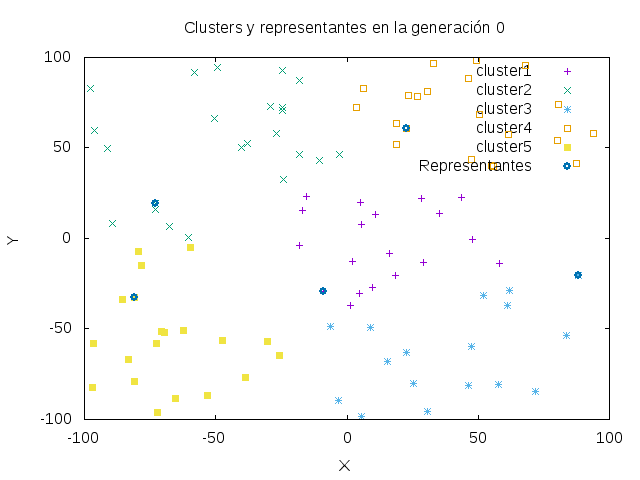
\includegraphics[width=0.7\linewidth]{graficos/0out}
\caption{Coste mínimo: 32.063385819971245}
\label{fig:0out}
\end{figure}

En esta primera generación de ideas aleatorias se tienen separados por colores cada uno de los clusters anteriormente dichos. Cada uno de ellos tiene un punto azul, el cuál es su representante de clase. Es la idea que, dentro de su cluster, tiene menor coste. Esos puntos será donde centraremos nuestra búsqueda y actuarán como punto de atracción.\\

\begin{figure}[H]
\centering
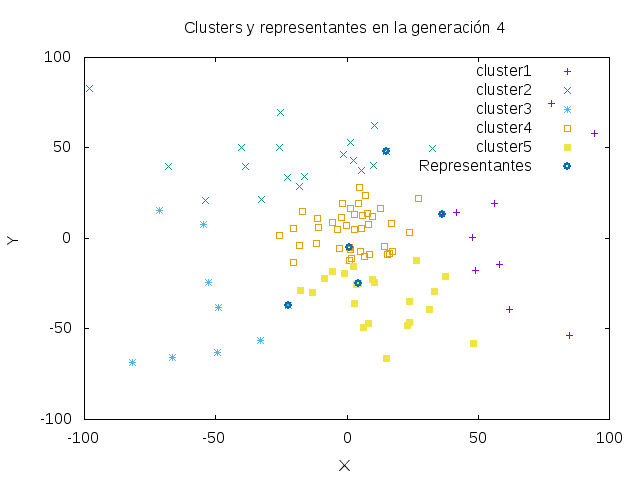
\includegraphics[width=0.7\linewidth]{graficos/4out}
\caption{Coste mínimo: 10.868608361185013}
\label{fig:1out}
\end{figure}

Tras unas cuantas generaciones vemos que se han agrupado ligeramente en el centro unos cuantos puntos (que es donde sabemos que la función de coste tiene un mínimo). Por último, en la última generación:\\

\begin{figure}[H]
\centering
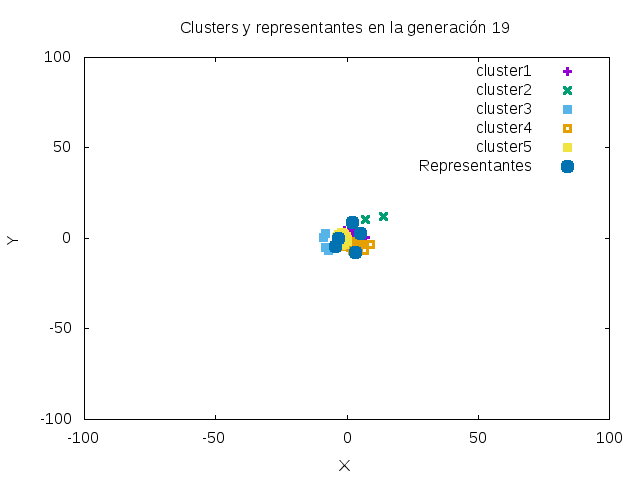
\includegraphics[width=0.7\linewidth]{graficos/19out}
\caption{Coste mínimo: 0.20025825415018517}
\label{fig:19out}
\end{figure}

se observa que se han agrupado todavía más en el centro. 


\section{Experimento y análisis de resultados.}

Para probar la bondad de este algoritmo vamos a compararlos con los resultados de la competición cec2014. Para empezar, aquí tenemos los resultados de nuestro algoritmo para las distintas dimensiones:\\

\textbf{Dimensión 10}

\begin{table}[htbp]
	\begin{center}
		\begin{tabular}{|l|l|}
			\hline
			Función & MejorCoste \\
			\hline \hline
			1 & 1183474.3628089789\\ \hline
			2 & 68864449.62907574 \\ \hline
			3 & 12052.281460498438 \\ \hline
			4 & 69.51174869048253 \\ \hline
			5 & 20.248590712702935 \\ \hline
			6 & 7.753179595914844 \\ \hline
			7 & 3.037059227484292 \\ \hline
			8 & 37.275446377989056 \\ \hline
			9 & 43.98963821630082 \\ \hline
			10 & 1000.5484210292489 \\ \hline
			11 & 1113.7294002188828 \\ \hline
			12 & 0.6969247915296819 \\ \hline
			13 & 0.307090955059266 \\ \hline
			14 & 0.48214180040963583 \\ \hline
			15 & 7.174151442472294 \\ \hline
			16 & 3.337923901207205 \\ \hline
			17 & 5020.6204587966295 \\ \hline
			18 & 1390.9914594921079 \\ \hline
			19 & 4.2737342582693145 \\ \hline
			20 & 418.4109712910604 \\ \hline
			
		\end{tabular}
		\caption{Datos obtenidos para el algoritmo BL}
		\label{tabla:Dimension10}
	\end{center}
\end{table}








\subsection{Análisis de resultados}



\subsection{Posibles mejoras de los algoritmos}


\newpage
\begin{thebibliography}{9}
	\bibitem{BSO} 2011 - BSO (IJSIR) -Brain Storm Optimization Algorithm\\
	
	\bibitem{smith} Smith, R.: The 7 Levels of Change, 2nd edn. Tapeslry Press (2002)\\
	
\end{thebibliography}


\end{document}





